\section{Orientation}
In order to draw a \rubik{} on the screen there are to things which are needed; the position of each \cubie{} and the orientation of each \cubie{}. This section will deal with the orientation of a \cubie{}.

The way to define an edge \cubie{} differs from the way to define a corner \cubie{}, which is why these to are dealt with separately.

\subsection{Corner Cubie}
A corner \cubie{} in a given \cubicle{} can ``sit'' in this \cubicle{} in one of three ways. See figure \ref{fig:orientation} for the the three different orientations of the white/blue/red corner \cubie{}.
Since each corner \cubie{} has one of each \facelet{} type -- one primary, one secondary, and one tertiary -- the orientation can be defined from where one of these \facelet{}s are positioned.
These different orientations can thereby be defined with an integer between 0 and 2.
0 if the primary \facelet{} of the \cubie{} is on the primary \face{}, 1 if the primary \facelet{} is on the secondary \face{}, and 2 if the primary \facelet{} is on the tertiary \face{}.

\begin{figure}[htb]
	\centering
		\subfloat[\myCaption{The white/blue/red corner is correctly oriented, which gives it the orientation value 0.}]{\label{fig:orientation:orientation0}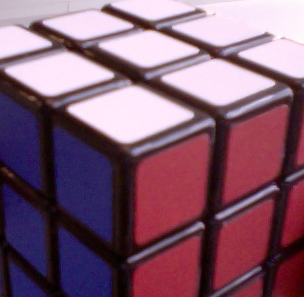
\includegraphics[width=0.28\textwidth]{input/pics/orientation0}}
		\hspace{0.02\textwidth}
		\subfloat[\myCaption{The white/blue/red corner is incorrectly oriented, the orientation value of this is 1 since the primary color is on a secondary face.}]{\label{fig:orientation:orientation1}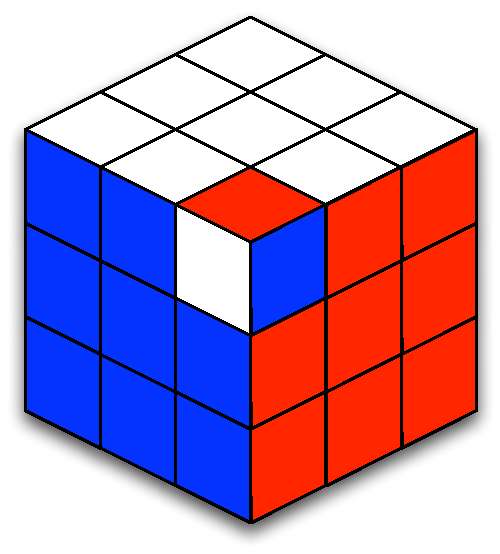
\includegraphics[width=0.28\textwidth]{input/pics/orientation1}}
		\hspace{0.02\textwidth}
		\subfloat[\myCaption{The white/blue/red corner is incorrectly oriented, the orientation value of this is 2 since the primary color is on a tertiary face.}]{\label{fig:orientation:orientation2}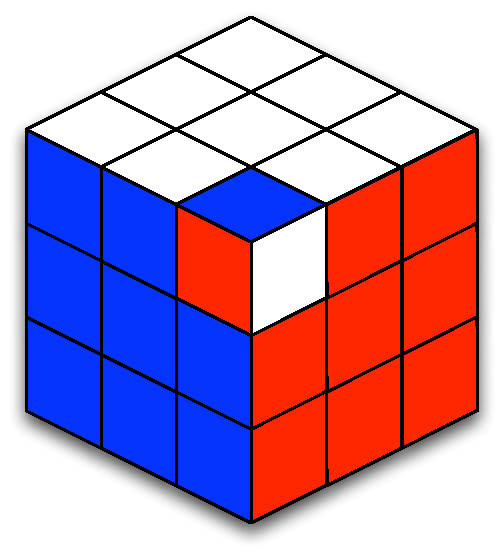
\includegraphics[width=0.28\textwidth]{input/pics/orientation2}}
		\caption{\myCaption{The three different orientation which the white/blue/red cubie can have. In these figures the white and yellow faces are primary, the blue and green are secondary, and red and orange are tertiary.}}
		\label{fig:orientation}
\end{figure}

In order to make it easier to draw the \rubik{} a secondary orientation is added. This orientation is defined from which \face{} the secondary \facelet{} is on.
This orientation is also defined from a integer between 0 and 2.
0 if the secondary \facelet{} of the \cubie{} is on the primary \face{}, 1 if the secondary \facelet{} is on the secondary \face{}, and 2 if the secondary \facelet{} is on the tertiary \face{}.
Note that a correctly oriented \cubie{} will have primary orientation 0 and secondary orientation 1.
It will also be easy to define a tertiary orientation of a \cubie{} by where the tertiary \facelet{} is positioned, but this will be redundant since the this integer always will have the value which the other orientations does not. E.g. the primary orientation is 0, the secondary orientation is 1, then the tertiary orientation must be 2.
See figure \ref{fig:orientationFlow} for a flowchart on how to find the primary and/or the secondary orientation of a corner \cubie{}.

\subsection{Edge Cubie}
The orientation of a edge \cubie{} can be defined with a boolean value; either it is correctly oriented or it is not.
This is easiest to see when the \cubie{} is in the right position e.g.
If the white/blue edge \cubie{} is in its correct \cubicle{} then it is correctly oriented if the white \facelet{} is on the white \face{} and the blue \facelet{} is on the blue \face{}.
The \cubie{} is wrongly oriented if the blue \facelet{} is on the white \face{} and the white \facelet{} is on the blue \face{}.

This raises the question: What is the orientation of a \cubie{} which is not in its correct \cubicle{}?
This was not to difficult with corner \cubie{}s because they always had a \facelet{} of each type, which an edge does not. An edge can be one of the following combinations of \facelet{} types: Primary/secondary, primary/tertiary, or secondary/tertiary. With this knowledge it is possible to simply look at the ``highest'' \facelet{}, meaning the \facelet{} with the highest rank.
The rank refers to the type of \facelet{}, where primary is the highest, secondary the second highest rank, and tertiary the lowest.
Then define the orientation as the following: If the highest \facelet{} of a \cubie{} is on the highest \face{}, then the \cubie{} is correctly oriented.
In order to stay in connection with corner \cubie{} the correct orientation of a \cubie{} is given the number 0 and the incorrect orientation the number 1.
Note that this is opposite to what is usually done in programming where 1 is true and 0 is false \cite{boolean2}.
See the flowchart in figure \ref{fig:orientationFlow}.

\begin{figure}[hbp]
	\centering
		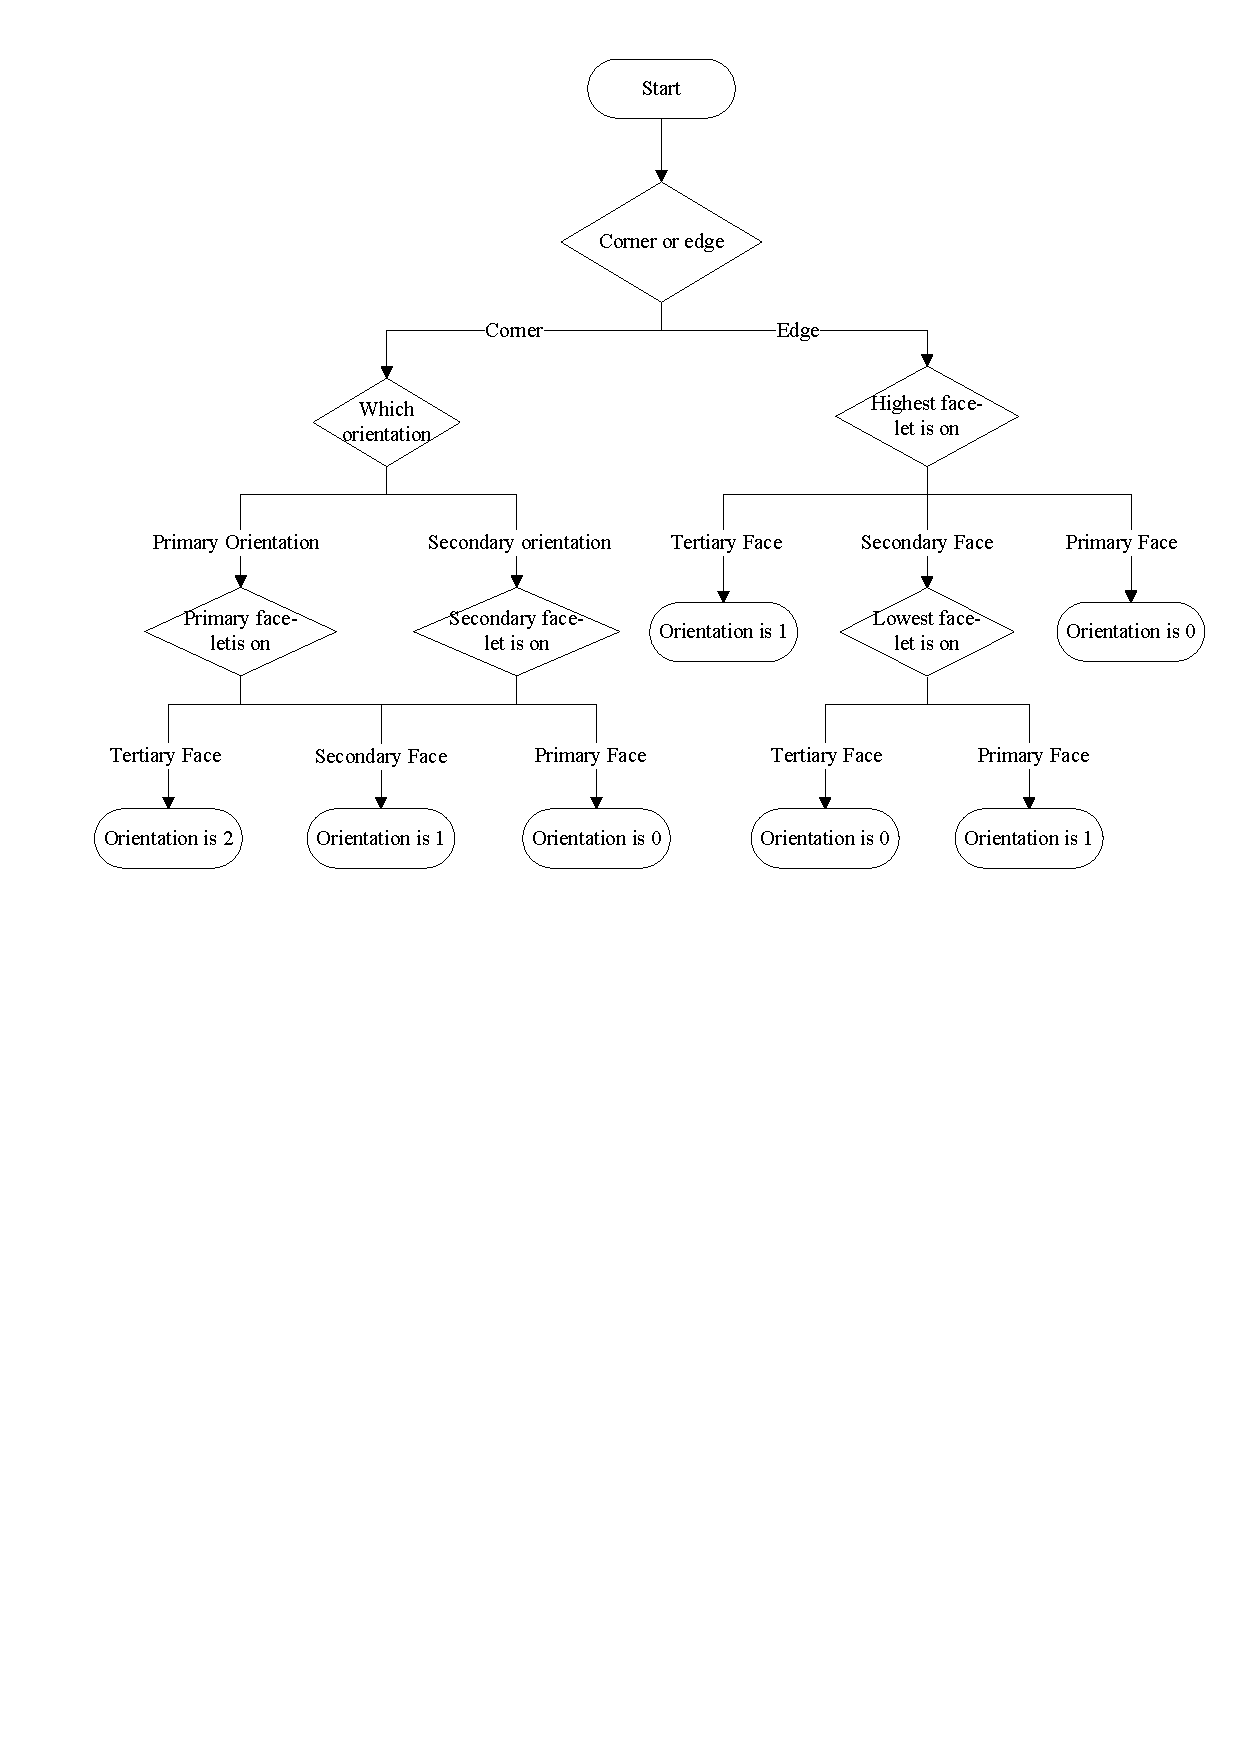
\includegraphics[width = \textwidth, trim = 10mm 120mm 0mm 10mm, clip]{input/pics/orientationFlow}
	\caption{\myCaption{Follow this flowchart to get the orientation of a cubie.}}
	\label{fig:orientationFlow}
\end{figure}
